\documentclass[tikz,border=4pt]{standalone}
\usepackage{amsmath}
\usepackage{xcolor}
\usepackage{xspace}
\usepackage{tikz}
\usetikzlibrary{arrows.meta,positioning}

\definecolor{caraprimary}{RGB}{30,60,120}
\definecolor{caraaccent}{RGB}{200,80,60}
\newcommand{\effnet}{EfficientNet-B0\xspace}

\begin{document}
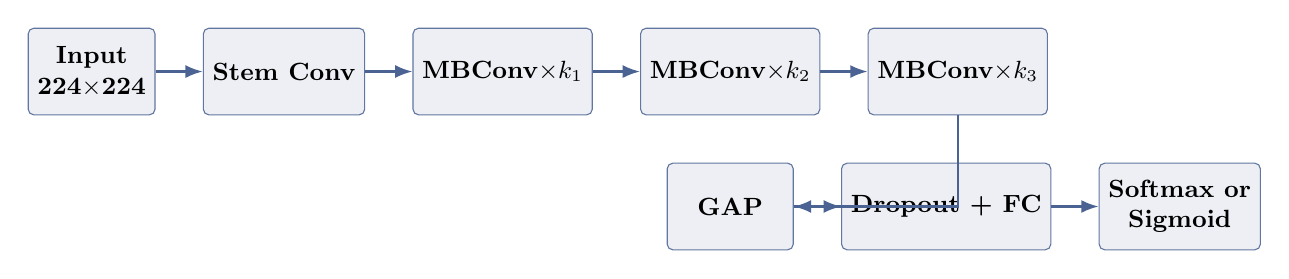
\begin{tikzpicture}[
    block/.style={rectangle, draw=caraprimary!70, fill=caraprimary!8,
        minimum height=1.1cm, minimum width=1.6cm, rounded corners=2pt,
        align=center, font=\small\bfseries},
    arrow/.style={-{Latex[length=2.2mm]}, thick, draw=caraprimary!80}]
\node[block] (in)   {Input\\224\(\times\)224};
\node[block, right=6mm of in]    (stem) {Stem Conv};
\node[block, right=6mm of stem]  (mb1)  {MBConv\(\times k_1\)};
\node[block, right=6mm of mb1]   (mb2)  {MBConv\(\times k_2\)};
\node[block, right=6mm of mb2]   (mb3)  {MBConv\(\times k_3\)};
\node[block, below=6mm of mb2]   (gap)  {GAP};
\node[block, right=6mm of gap]   (fc)   {Dropout + FC};
\node[block, right=6mm of fc]    (out)  {Softmax or\\Sigmoid};

\draw[arrow] (in) -- (stem);
\draw[arrow] (stem) -- (mb1);
\draw[arrow] (mb1) -- (mb2);
\draw[arrow] (mb2) -- (mb3);
\draw[arrow] (mb3.south) |- (gap.east);
\draw[arrow] (gap) -- (fc);
\draw[arrow] (fc) -- (out);
\end{tikzpicture}
\end{document}
